\chapter{Discussion}
This chapter is an extension to the article with additional result analysis and a deeper discussion of how they support the proposed model and what insights they give to support its use for other applications.

\section{A detailed look at obfuscation method information}
\begin{figure}
	\centering
	
	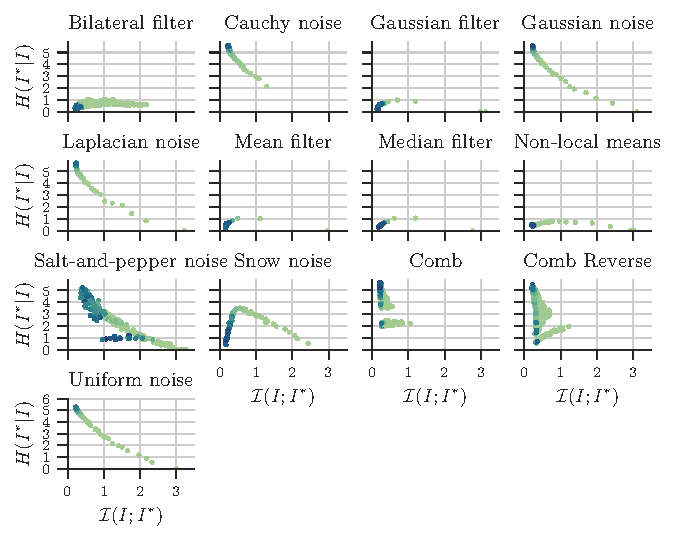
\includegraphics[width=1\textwidth]{figures/results/individual}
	
	\caption{Plot of mutual information and conditional information response for individual filters. Note that these distributions are estimated from the entire image, producing less noisy results than the ones presented in the article.}\label{fig:individual}
\end{figure}

\Cref{fig:individual} shows mutual information and conditional entropy for each filter separately. This makes the distinction between them even more noticeable. 

The noise methods, except snow and salt-and-pepper, all follow an almost straight line, "converting" mutual information into conditional entropy. \Cref{fig:individual-entropy} is similar, but with the output image entropy as its x-axis. From this figure it is clear that for all noise methods, the increase in conditional information is roughly proportional to the increase in entropy, but not at a one-to-one scale. As shown in \cref{eq:entropy-law}, this necessitates a loss in mutual information, i.e. $\mathcal{I}(I^*;I) = H(I^*) - H(I^*|I)$. Since the entropy and conditional entropy are roughly linearly correlated for the noise-based methods, we have $H(I^*) \approx \alpha H(I^*|I) + H(I)$ and as a consequence, the mutual information can be expressed as a function of the conditional entropy and the entropy of the original image 
\begin{align*}
\mathcal{I}(I^*;I) \approx (\alpha-1)H(I^*|I) + H(I).
\end{align*}
This is of course only an approximation.

The snow method has a sudden drop in conditional information which is caused by its definition. At low densities, snow increases conditional entropy because the randomly placed pixels adds high gradient components. At higher densities however, the fact that only the value $127$ is used for pixels starts to decrease the entropy significantly. The uniform snow method is susceptible to the same effect when gaussian variance is low and \todo{what about this?}

\begin{figure}
	\centering
	
	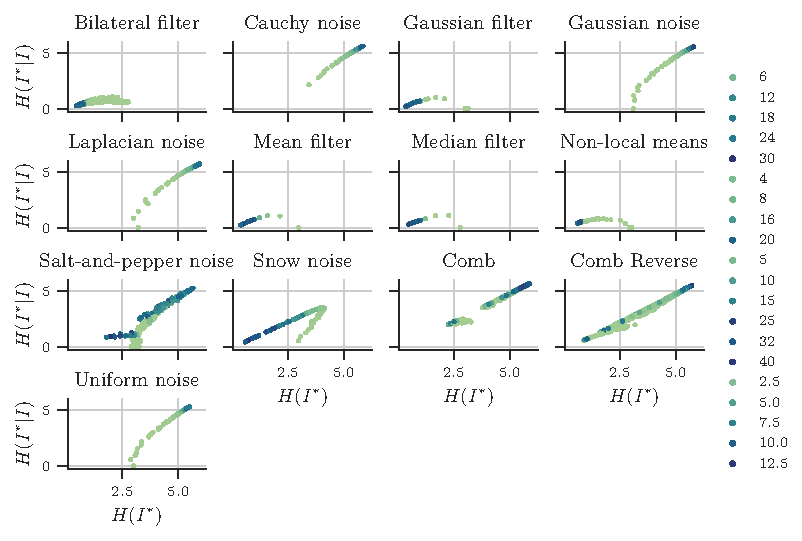
\includegraphics[width=1\textwidth]{figures/results/individual-ent}
	
	\caption{Plot of entropy of the obfuscated images and conditional information response for individual filters.}\label{fig:individual-entropy}
\end{figure}

The filter-based methods behave as explained in the article and only significantly impacts mutual information. The combination methods, and especially Comb, is worth investigating further. \Cref{fig:comb} uses the same axes as \cref{fig:individual} but displays only data from the Comb method and with the colours indicating the three parameters in the respective plots. The scale parameter, $\gamma$, correlates directly with the value of conditional entropy as expected. The generally lower mutual information values are likely caused by a narrower band of parameters used for the experiment due to time considerations. It therefore seems clear that the diagonal bands visible in the figures corresponds to the response caused by the bilateral filter. It correlates highly with the color variance parameter $\sigma_c$ but is seemingly independent from the spatial parameter $\sigma_s$. This effectively means that only small values of $\sigma_s$ is needed.

\begin{figure}
	\centering
	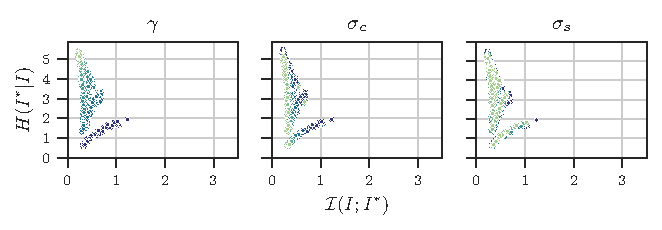
\includegraphics[width=1\textwidth]{figures/results/comb}
	\caption{}\label{fig:comb}
\end{figure}
\todo{Discuss camera effects}

\subsection{Filters and gradient entropy}
Although the approach to filtering has been argued extensively in the article, it did not show how visually appropriate the gradient entropy is compared to a simple intensity entropy. \Cref{fig:delentropy} shows a number of sample images for which both the intensity histogram and gradient histograms have been calculated. It is visually very clear how the gradient histogram and its entropy corresponds with the visually perceived image complexity.

\begin{figure}
    \centering
    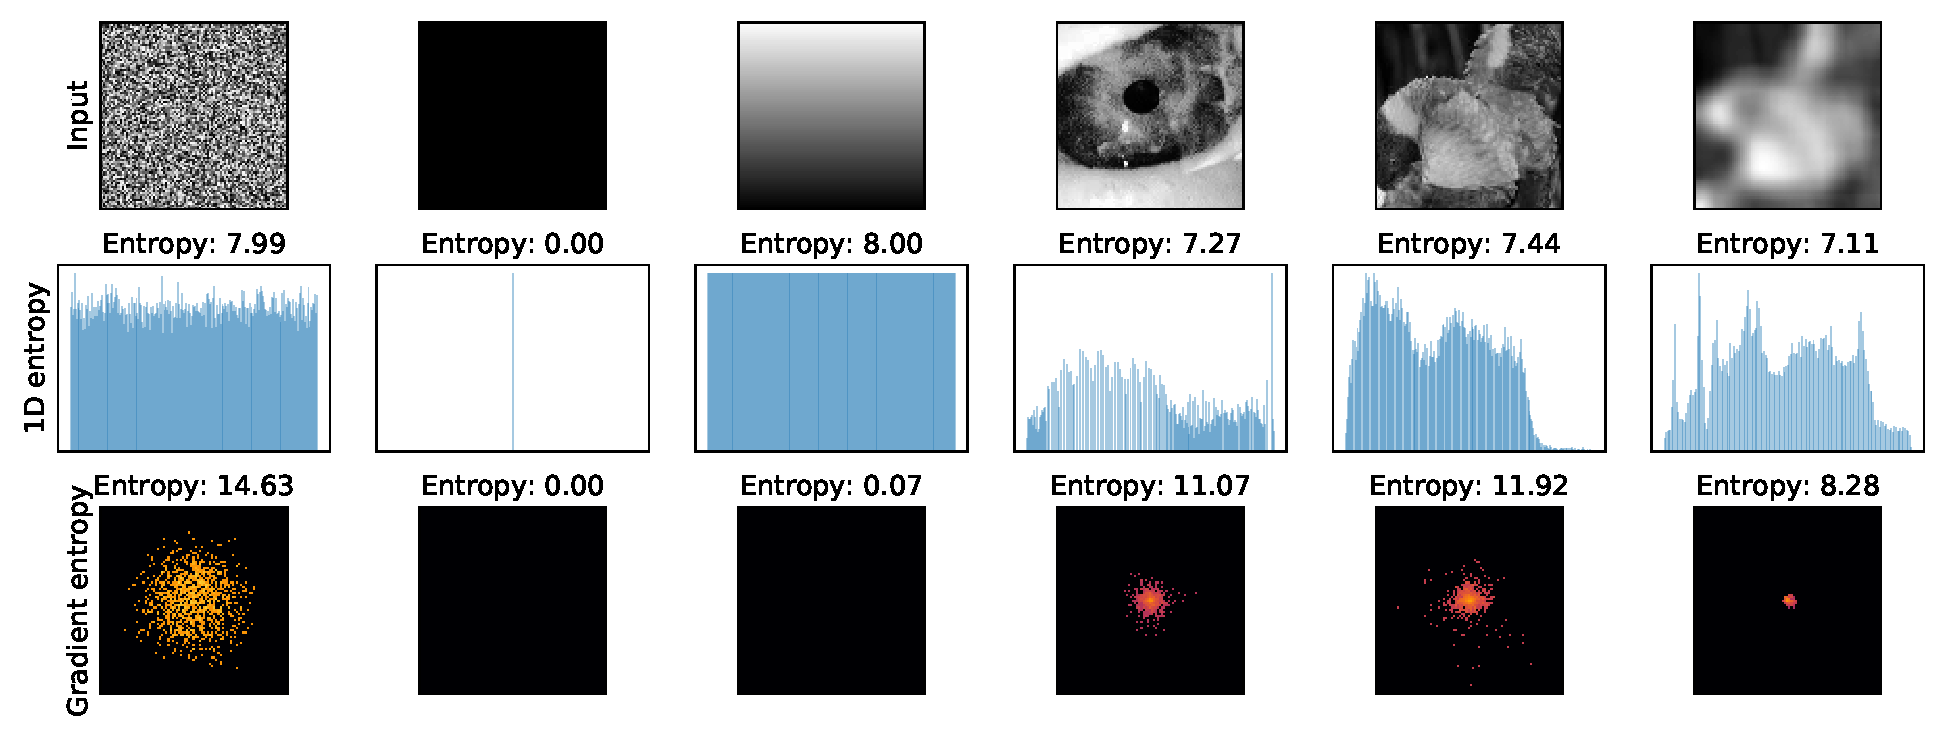
\includegraphics[width=1\linewidth]{figures/results/delentropy}
    \caption{Comparison between entropy of intensity and gradient histograms for a number of image samples.}
    \label{fig:delentropy}
\end{figure}

Sample applications of the proposed obfuscation methods are shown in \cref{fig:filters} where the same visual correlation is still clearly present. The Comb method is also visually indicative of its effectiveness as an obfuscation method because of the clear blurring of eye details while retaining a layer of noise. The parameters used in this example are exaggerated to increase the perceivability of the effects.

\begin{figure}
    \centering
    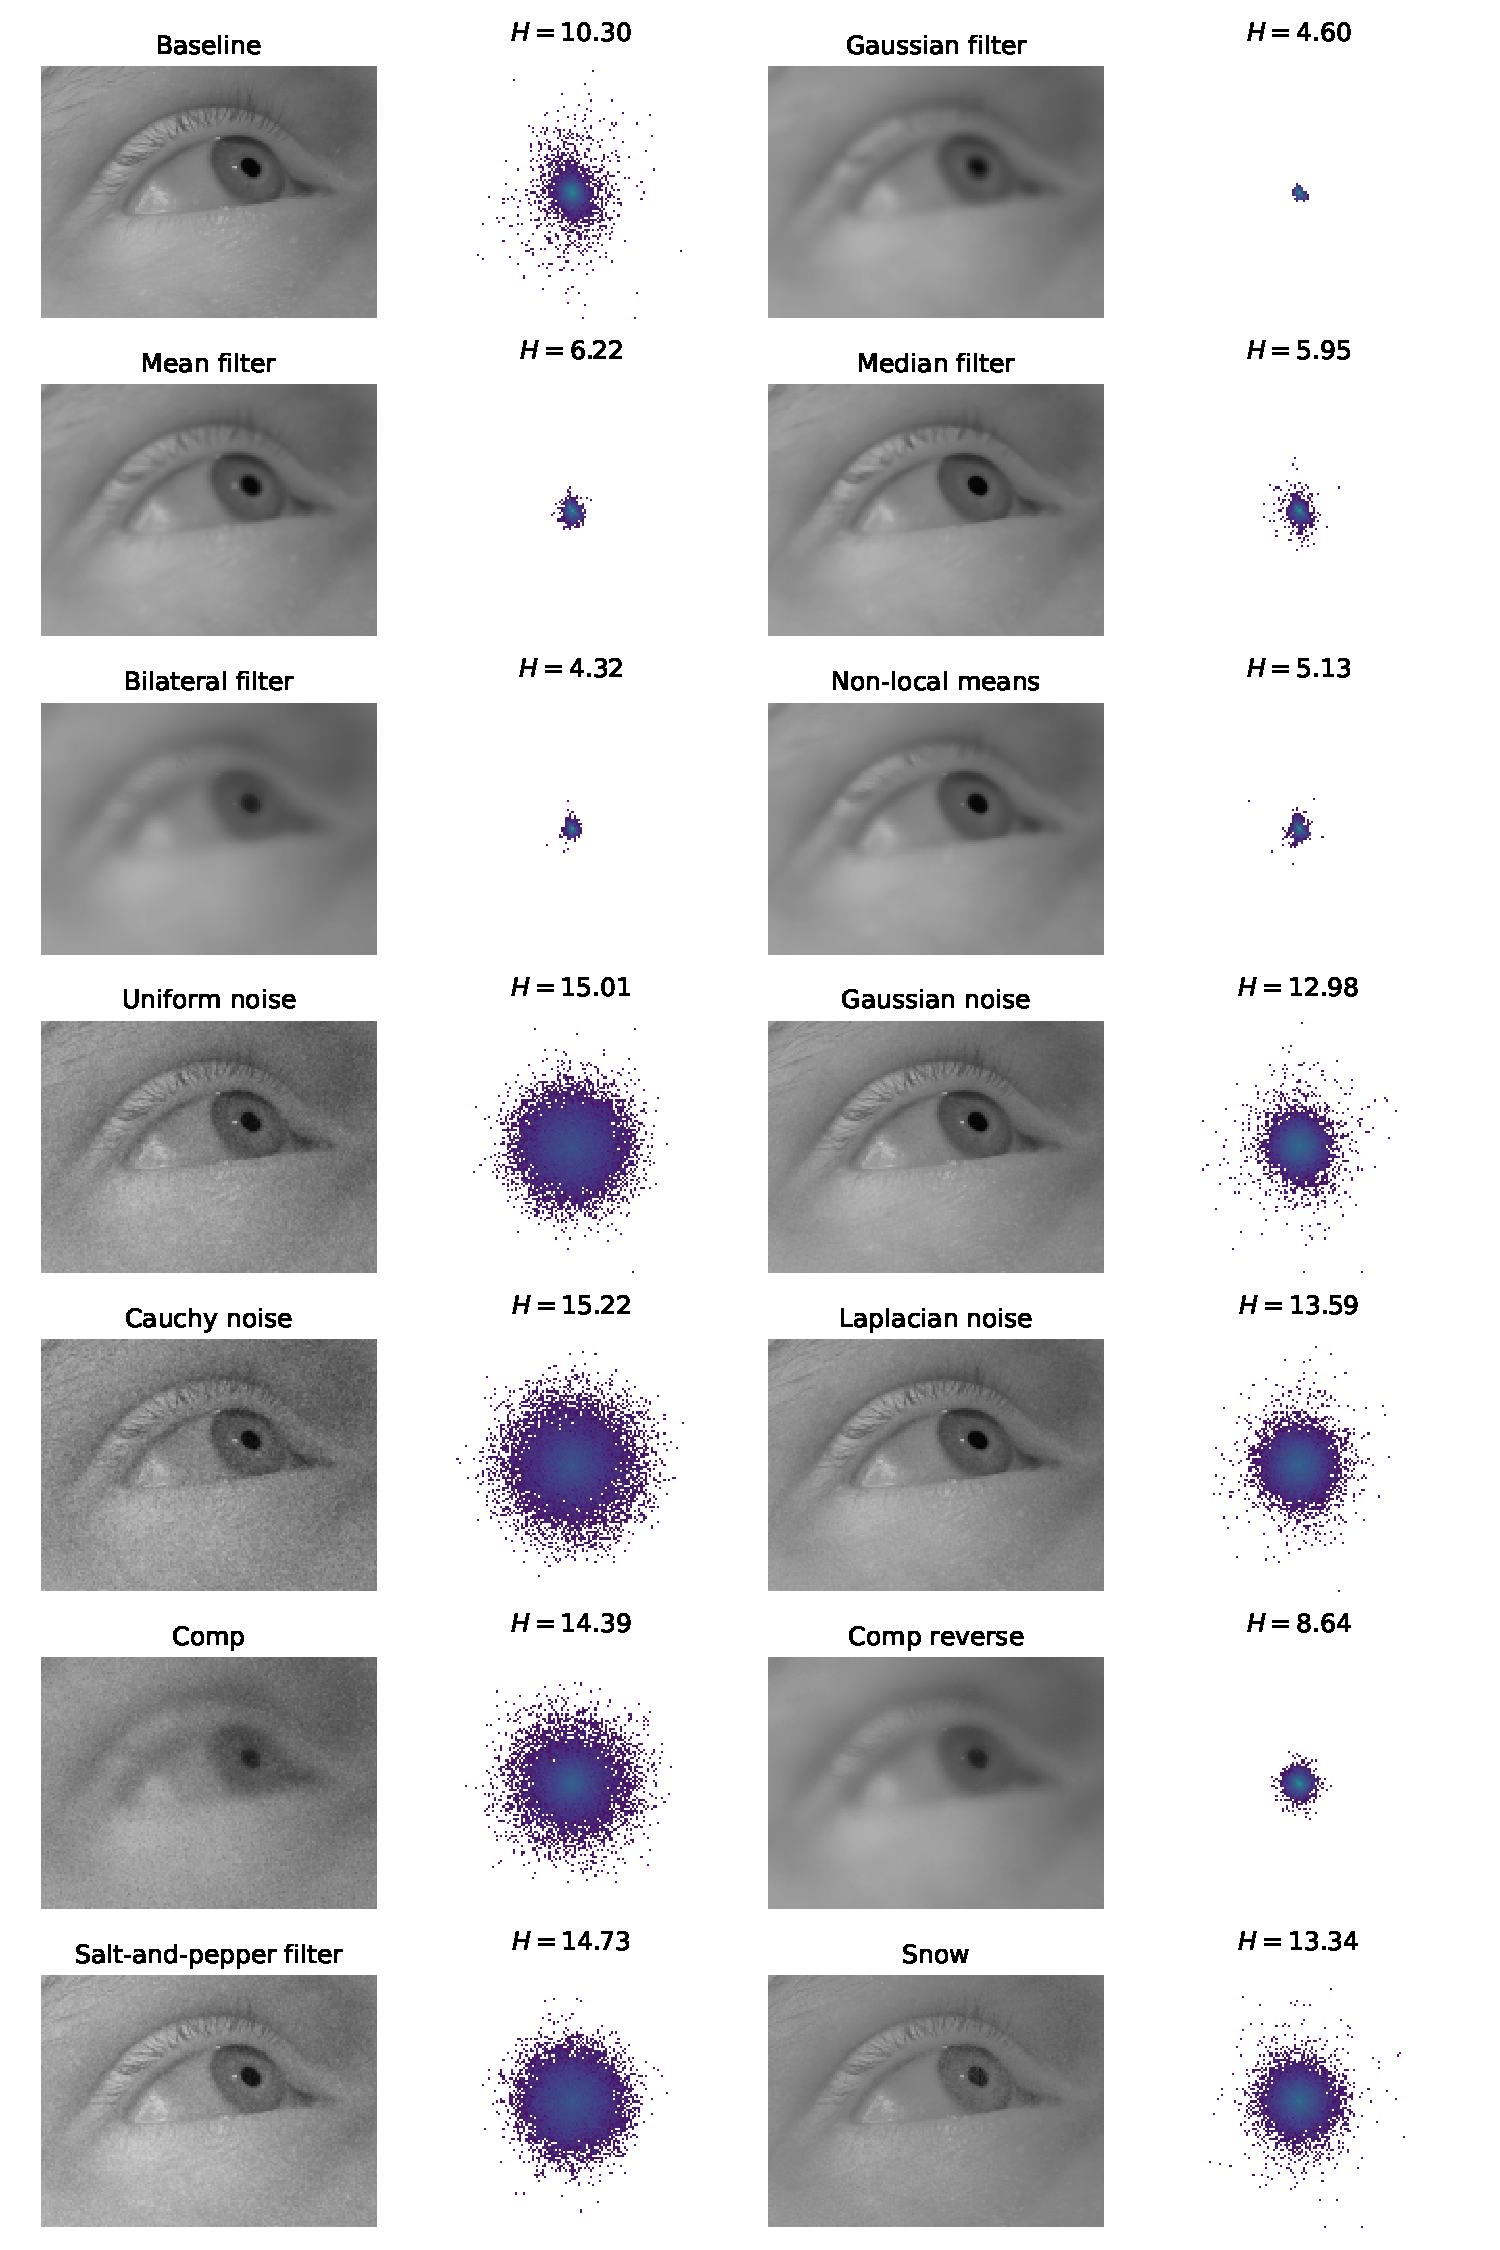
\includegraphics[width=0.85\linewidth]{figures/results/filter_effect.pdf}
    \caption{Shows effect of applying the proposed filters. The heat-maps show the corresponding gradient histogram.}
    \label{fig:filters}
\end{figure}


%Specifically, one of the previous studies tested a Gaussian filter (and optical defocus) \parencite{BRENDAN_BLUR} for obfuscation based on the assumption that the lowest frequency wavelength of the pupil edge would be enough to enable robust gaze estimation. The problem with the Gaussian filter is that it is a low-pass filter, i.e. it removes high-frequency components. Since sharp edges are only sharp because of these, a Gaussian filter makes images look blurry and unsharp as a result. The effect on the image in (FIG) is shown in (FIG)\todo{do it}, where a Gaussian filter with $\sigma=5$ has been applied. Clearly, the gradient at the edge has been smoothed considerably. The reason the study still reports favourable results is that the gaze-estimation algorithm is likely robust to at least some degree of edge blurring.

%A smarter approach is to consider not just the spatial neighbourhood but the intensity as well. 

\section{Eye information process model generalisation}\todo{ikke klart hvem der siger det...}
For the model and methodology presented in this thesis to be useful, it has to somehow be relevant to the way this category of problems are perceived and to how they are evaluated. For the specific application of iris obfuscation, this has been argued extensively in the article. At an abstract level, the model is used to understand the problem of iris obfuscation and for proposing reasonable and interesting solution candidates. At a concrete level, the information-based metrics and methods derived for calculating them for images showed a high correlation with the observed iris recognition accuracy.

The definition of the model itself as a Bayesian network or as a communication system is an expression of the similarity of image and signal manipulation operations and, by extension, of obfuscation methods in general. The optimisation goal defined for iris obfuscation is thus the same for any other obfuscation problem. The gaze signal itself contains information that has been shown to reveal multiple properties of the recorded subject and is therefore an obvious candidate for using the model. The model and methodology presented here can be applied directly. 

If applied to other problems, results become easier to analyse and compare, and the methodology itself will develop which might provide additional insight into already published material. 

\section{Differential privacy}
Differential privacy is too strict to be a realistic measure for proving privacy bounds for obfuscation tasks. Specifically, only low privacy-bounds are achievable by the application methods proposed so far in the literature. I here present the argument that this is caused by the properties of differential privacy when applied in this domain. Differential privacy is simply a measure of how much a random function impacts the predictability of changing a single element in a set of data points, e.g. an image. Formally, a random function $\mathcal{K}$ is $\epsilon$-differentially private if
\begin{align}
	P[\mathcal{K}(D_1)\in S] \leq \exp{\epsilon} P[\mathcal{K}(D_2)\in S],
\end{align}
for all subsets $S$ of the image of $\mathcal{K}$ and all datasets $D_1$, $D_2$ that differ in at most one element \parencite{dwork2006differential}. In other words, a differentially private function decreases the output's dependence on individual data points since this dependence can be used to infer the original data points.

Differential privacy measures for images have been proposed by \parencite{fan2018image}. Importantly, their extension from single pixel changes to neighbourhoods, come with a proportional increase in $\epsilon$ for the same amount of randomness, i.e. for a neighbourhood of $n$ pixels, the privacy should be $\epsilon/n$ to achieve the same level of protection as when a single element is changed. The solution presented in this study suggests an aggressive downsampling using averaging to achieve reasonable levels of noise. Specifically, for an image with pixel intensities in the range $0-255$, and using laplacian noise, the scale parameter is $\frac{255n}{b^2}$ where $b$ is the side length of grid cells defining regions to be averaged. Since laplacian noise has a variance of $2s^2$ where $s$ is the scale, even a low-resolution image of $100\times 10$ pixels (the size used for polar iris images in this work) would require laplacian noise with a variance of $\approx 130\times 10^9$ thus rendering the image practically unusable.

The method proposed in \parencite{BRENDAN_SNOW} does, however, use a weaker form of differential privacy allowing an extra constant term $\delta$ which signifies a probability of leaking information. They prove that $\delta$ has a maximum of $0.5$ for the snow method which means that each pixel has $50\%$ chance of a leak. However, as presented in \cref{sec:methods}, the method can easily be defeated if multiple samples are available. Additionally, even with a single sample, the method shows only moderate effectiveness at preventing recognition with high precision at low recall values. 

In conclusion, differential privacy is not suitable for determining the security of obfuscation methods due to their high sensitivity and the large areas of pixels that need to be secured. As a final note, this criticism does not concern the aggregation based attempts at differential privacy in eye-tracking mentioned in the article. %Instead it is 
 differential privacy has been shown to be highly effective in other eye-tracking privacy tasks where aggregation is involved (REFS).

\todo{Try to add the rest here}
% Instead, definitions should be derived from a

%\begin{definition}[Privacy]
%Let $S$ be an eye information signal and $\bar{S} \subseteq S$ a subset describing the sensitive data. 

%Let $\mathcal{A}$ be an arbitrary function for inferring 
%Given an arbitrary information extraction function $\mathcal{A}$, an obfuscation function $\mathcal{O}$, and a signal $S$, the privacy strength of $\mathcal{O}$ is defined as
%\begin{align}
%	P[\mathcal{A}(\mathcal{O}(S)) \cup \bar{S} \neq \empty] \leq \rho,
%\end{align}
%for an arbitrary threshold $\rho$ and for any $\mathcal{A}$.
%\end{definition}























